\begin{frame}
	\frametitle{Curvas en Variedades}
	\begin{definition}[Curva en variedades]
		Sea $M$ una variedad suave, diremos que $\gamma$ es \textbf{una curva suave} sobre $M$ si $\gamma: [a,b] \to M$ es un mapa suave.
	\end{definition} \pause

	\begin{definition}[Velocidad de una curva]
		Sean $\gamma: [a,b] \to M$ una curva suave, $t_0 \in [a,b]$ y $(U,\phi)$ una carta suave que contiene a $\gamma(t_0)$. Definimos la \textbf{velocidad de $\gamma$ en $t_0$} como el vector tangente:
		\[
			\gamma'(t_0) = \sum_{i=1}^{n} \frac{d\gamma_i(t_0)}{dt} \partial \phi_{i} \big|_{\gamma(t_0)}
		\]
	\end{definition}
\end{frame}

\begin{frame}
	\frametitle{Curvas en Variedades}
	\begin{figure}
		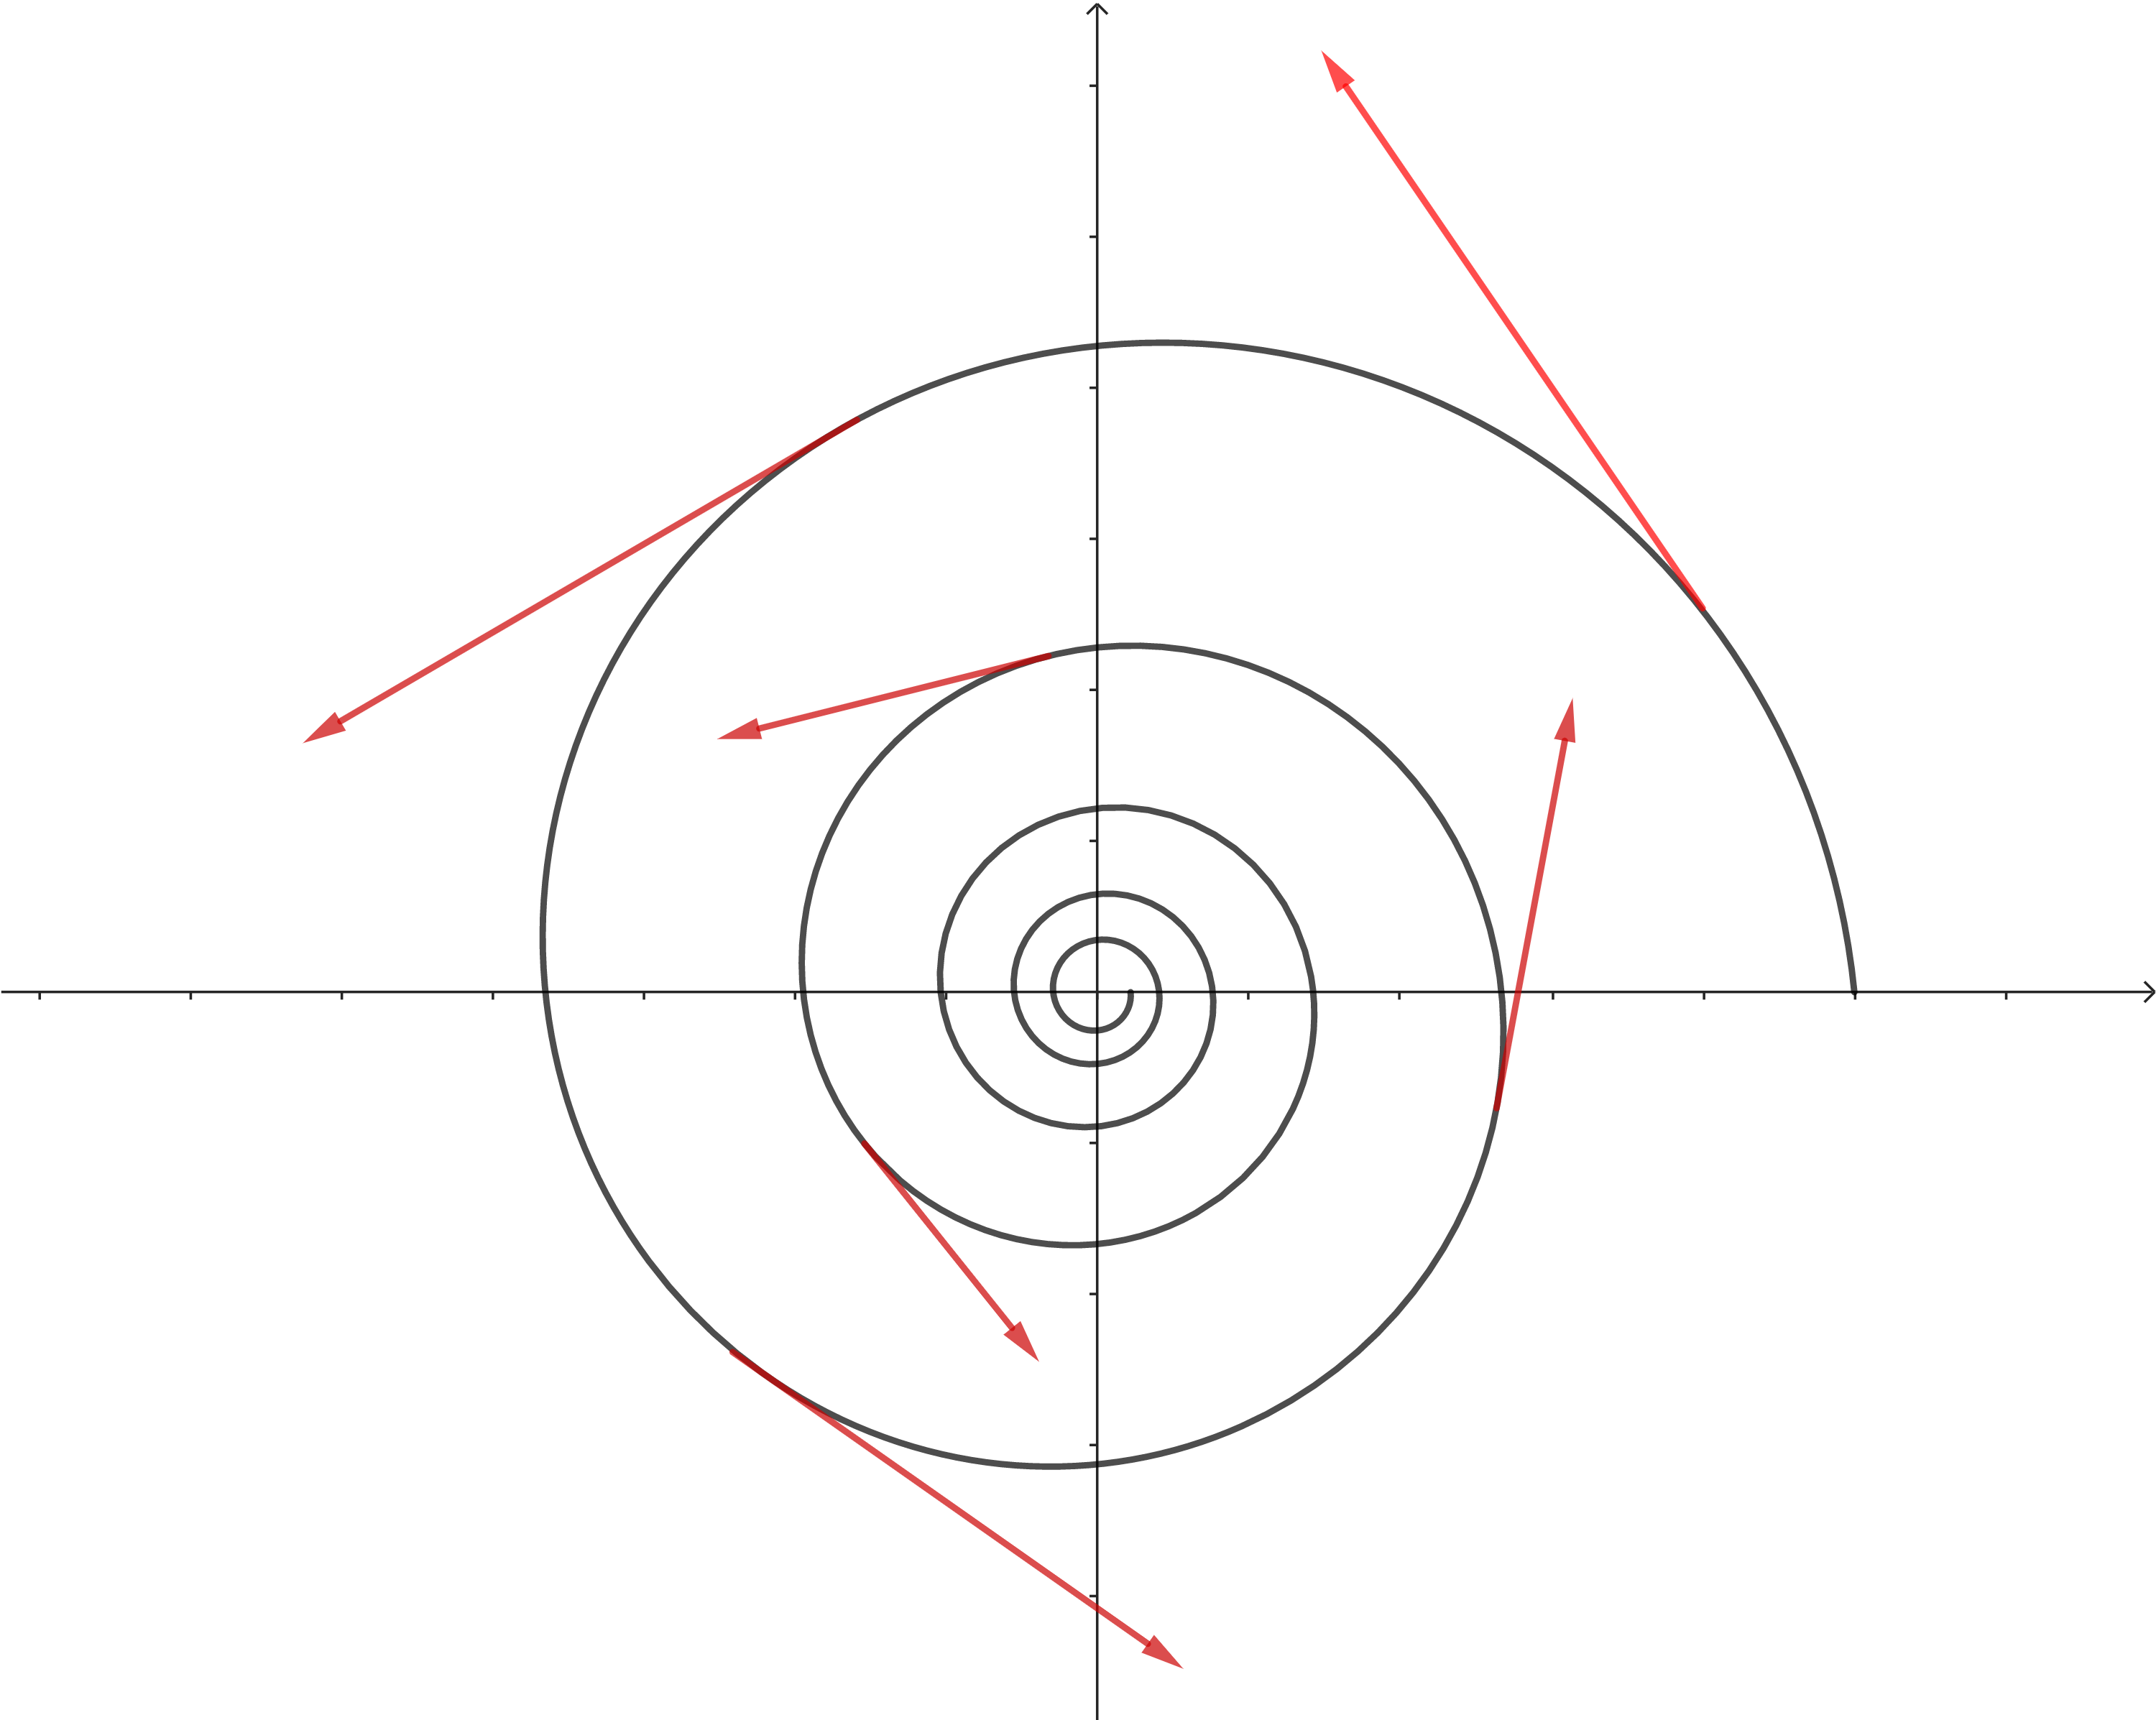
\includegraphics[scale=2.5]{Figuras/CurvaLogaritmica.png}
		\caption{Ejemplo de una curva en el plano con algunos vectores tangentes.}
	\end{figure}
\end{frame}

\begin{frame}
	\frametitle{Conexión Afín}
	\begin{definition}[Conexión afín]
		Una \textbf{conexión afín} en $M$ es un mapa bilineal:
		\[
			\nabla: \mathfrak{X}(M) \times \mathfrak{X}(M) \to \mathfrak{X}(M),
		\]\pause
		el cual cumple las siguientes dos propiedades:
		\begin{itemize}
			\item $\nabla$ es lineal en su primera coordenada con respecto al anillo de funciones suaves.
			      \[
				      \nabla(fX + Y, Z) = f\nabla(X,Z) + \nabla(Y,Z)
			      \]\pause
			\item $\nabla$ cumple la siguiente regla del producto:
			      \[
				      \nabla(X,fY) = X(f) Y + f\nabla(X,Y)
			      \]
		\end{itemize}
	\end{definition}
\end{frame}


\begin{frame}
\begin{center}
	\begin{figure}[h]
		\centering
		\begin{subfigure}{0.30\textwidth}
			\centering
			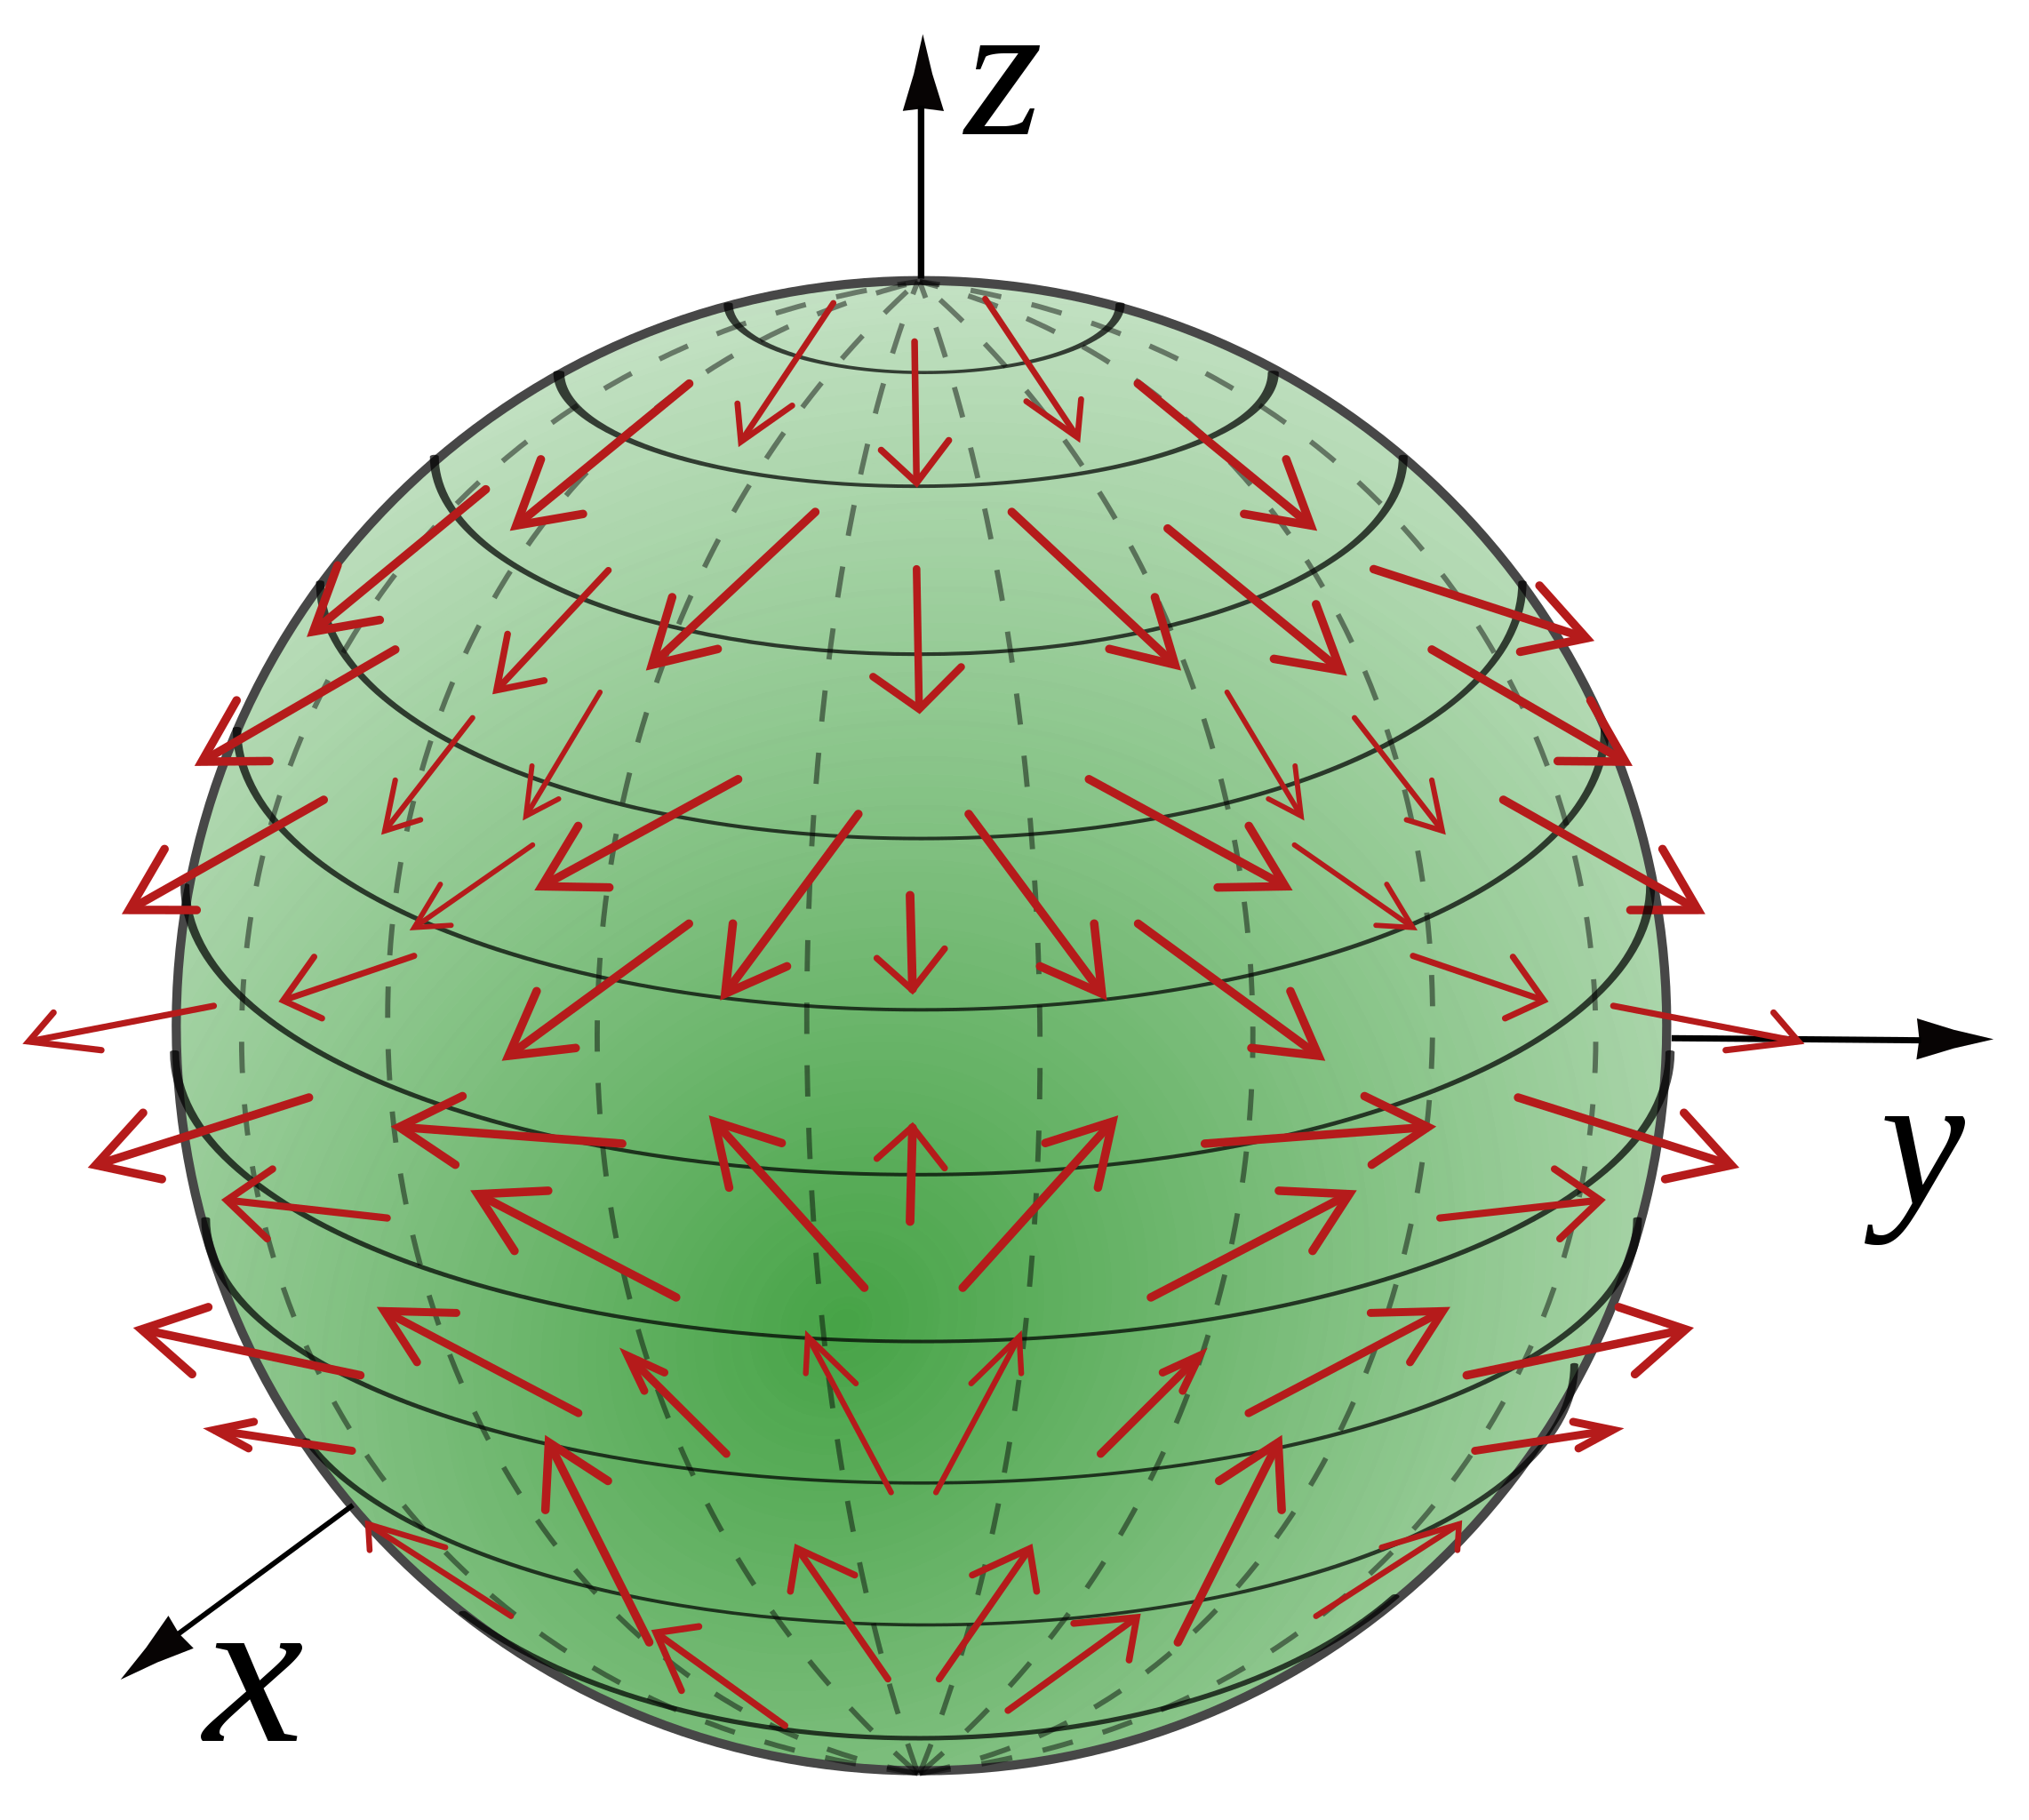
\includegraphics[scale=0.065]{Figuras/Vector_sphere.svg.png}
		\end{subfigure}
		\hspace{50pt}
		\begin{subfigure}{0.30\textwidth}
			\centering
			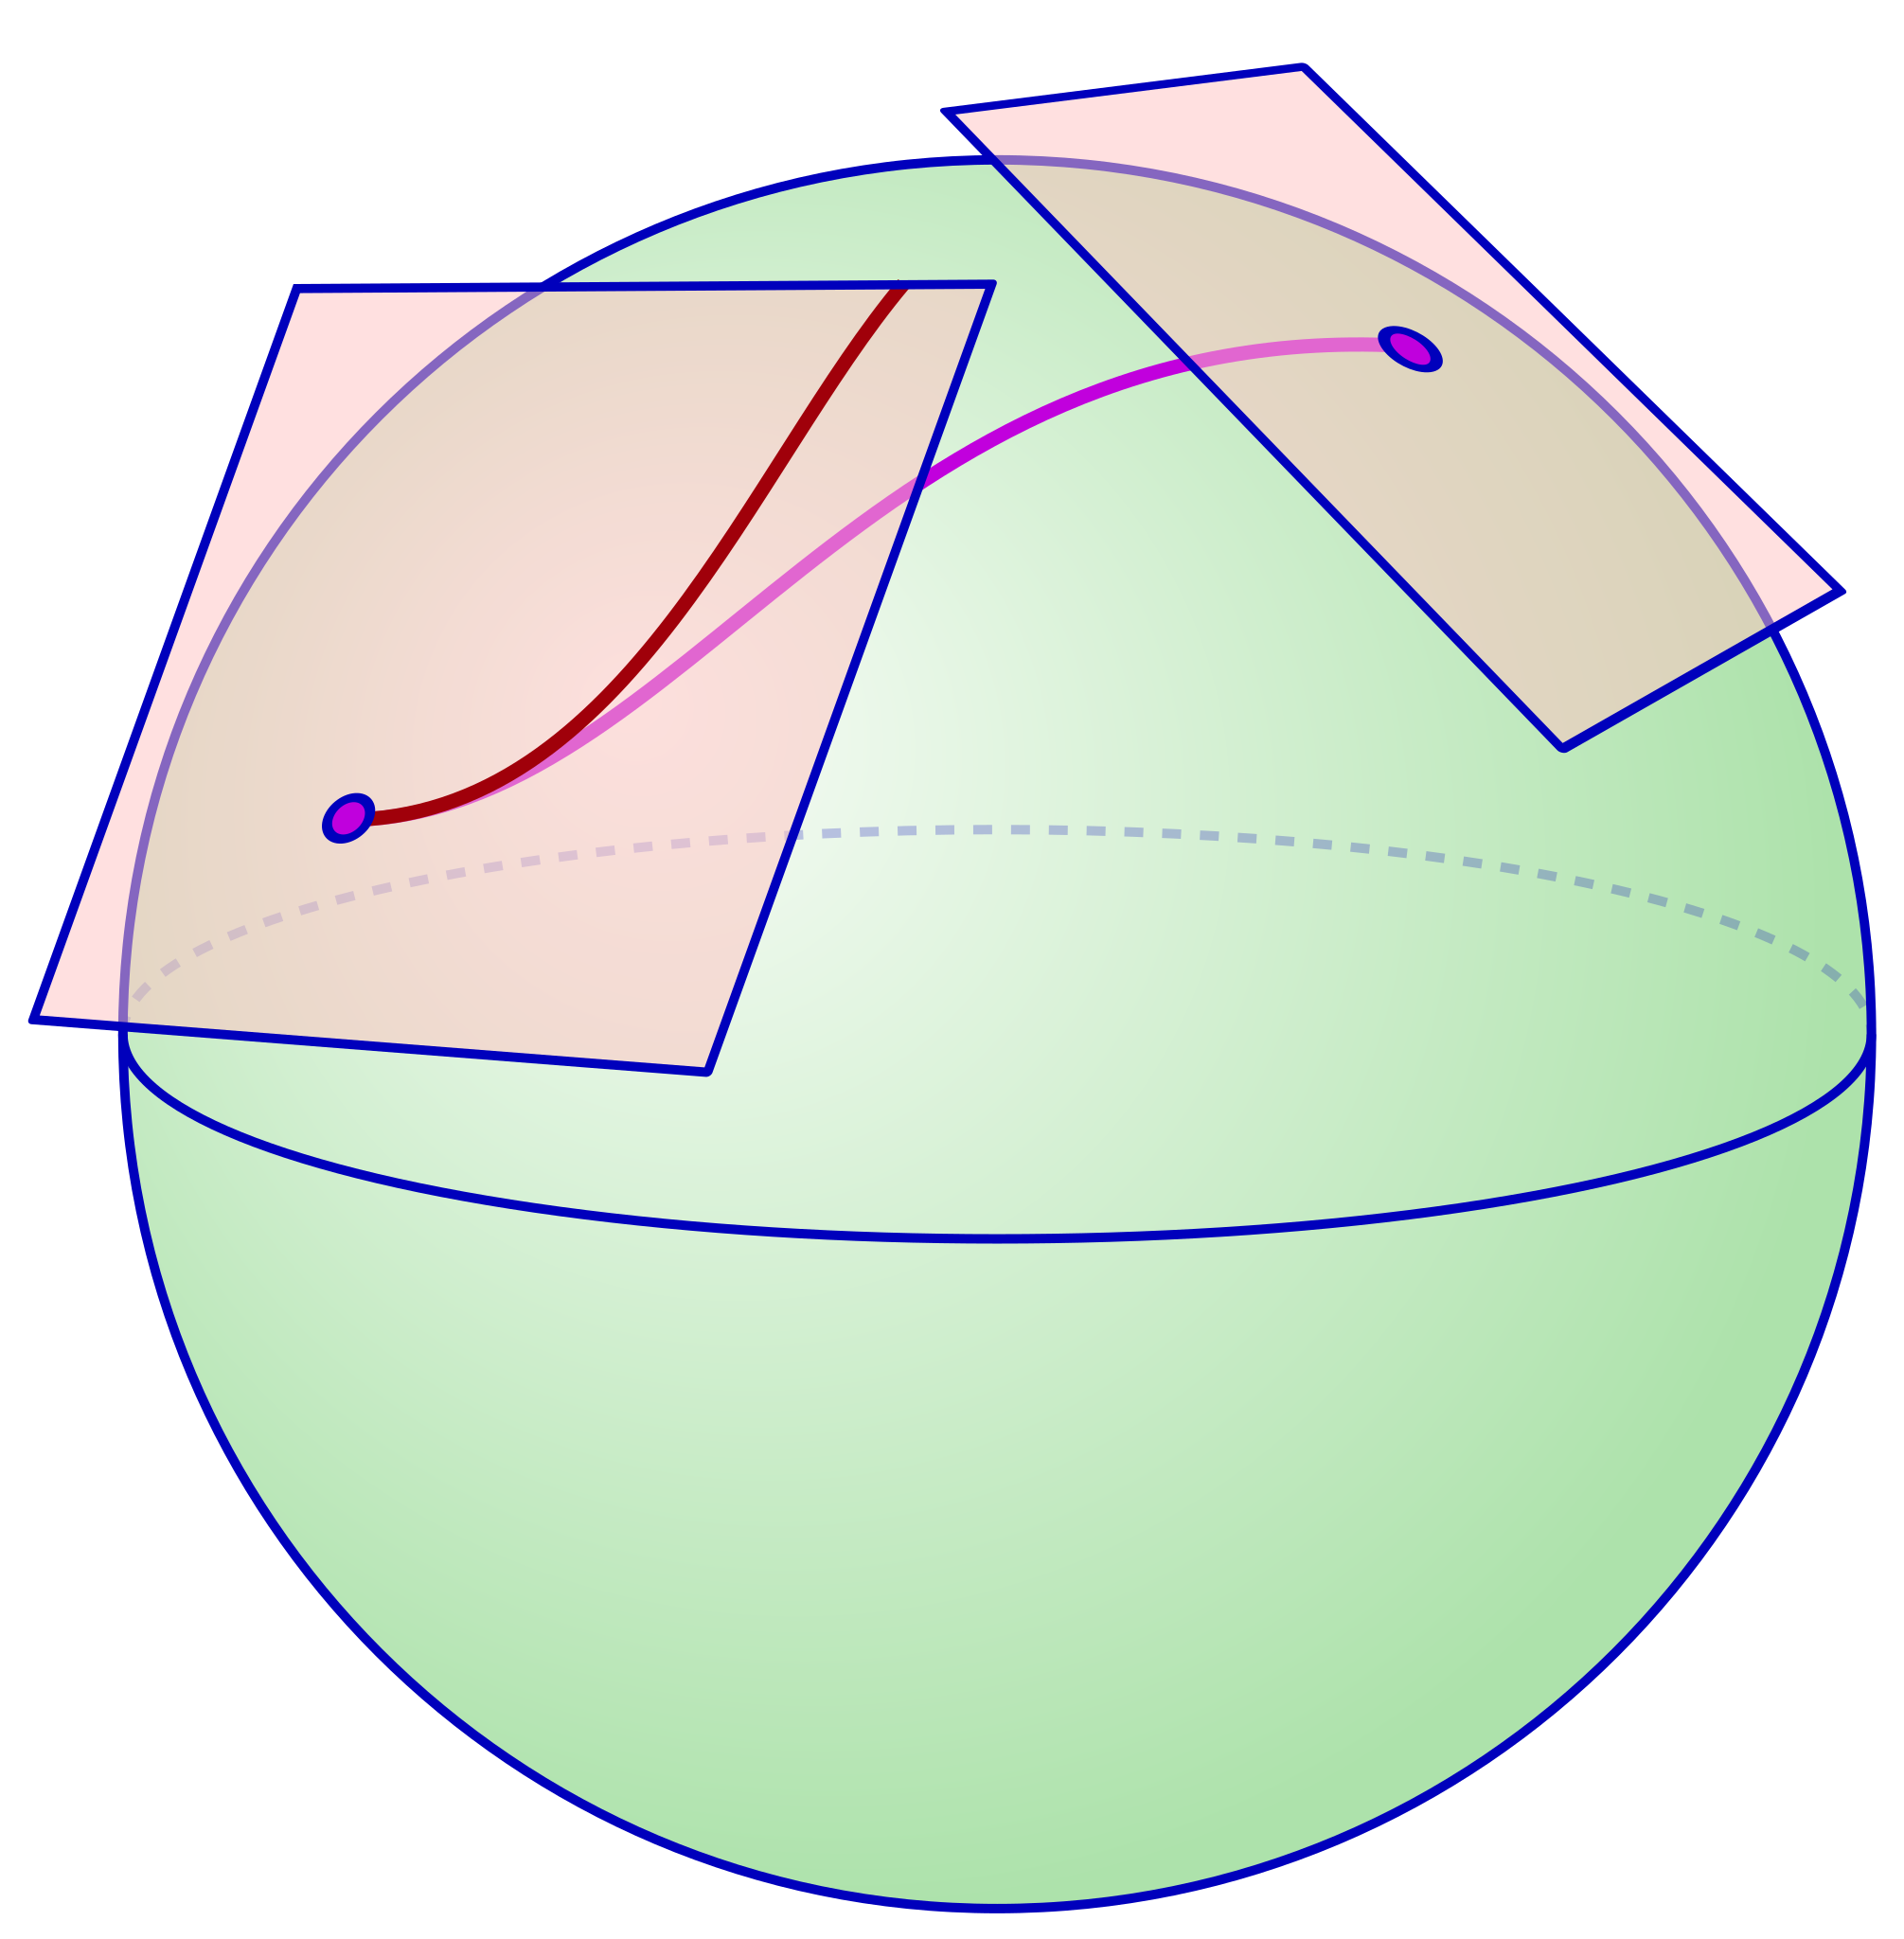
\includegraphics[scale=0.065]{Figuras/TransporteParalelo.png}
		\end{subfigure}
		\caption{Representación de una conexión afín en la esfera}
	\end{figure}
\end{center}
\end{frame}

\begin{frame}
	\frametitle{Conexión Afín}
	Usualmente se denota a la conexión afín $\nabla(X,Y)$ como $\nabla_{X}Y$ y se le llama \textit{la derivada covariante de $Y$ en la dirección de $X$}.

	\pause

	\vspace{12pt}

	De manera local la derivada covariante puede ser expresada como:
	\[
		\nabla_{X}Y = \sum_{k=1}^{n} \left(
		X(Y_{k}) + \sum_{i=1}^{n}\sum_{j=1}^{n} \Gamma_{ij}^{k} X_{i}Y_{j}
		\right) \partial_{k},
	\]\pause
	En la ecuación anterior $\Gamma_{ij}^{k}$ son $n^{3}$ funciones suaves, a las cuales se les llama los \textit{símbolos de Christoffel}. \pause En una variedad Riemanniana los símbolos pueden ser obtenidos por la ecuación:
	\[
		\Gamma_{ij}^{m} = \frac{1}{2} \sum_{k=1}^{n} (\partial_{i} g_{jk} + \partial_{j}g_{ji} - \partial_{k}g_{ij}) g^{km}
	\]
\end{frame}
